\chapter{PROCEDIMIENTO}

\section{Red de Pares: Computador-Computador}

\begin{caja}[]{
 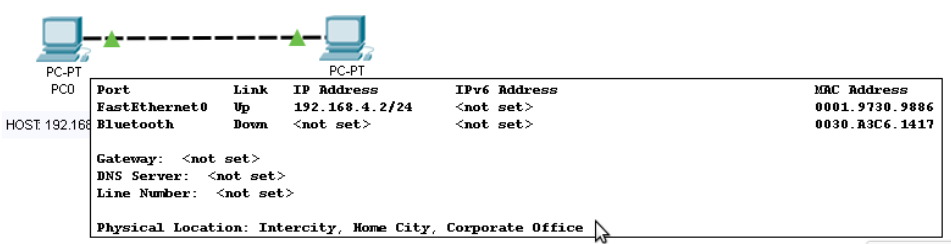
\includegraphics[scale=0.43]{conputador} }
 \end{caja}
 
\begin{definicion}[]{
La configuraci\'on de este tipo de conexi\'on es sencillo; lo \'unico que debemos de hacer es establecer las direcci\'ones ip de cada host.}
\end{definicion}


\subsection{Simule el env\'io de un PDU entre los dispositivos a fin de verificar la conectividad.}
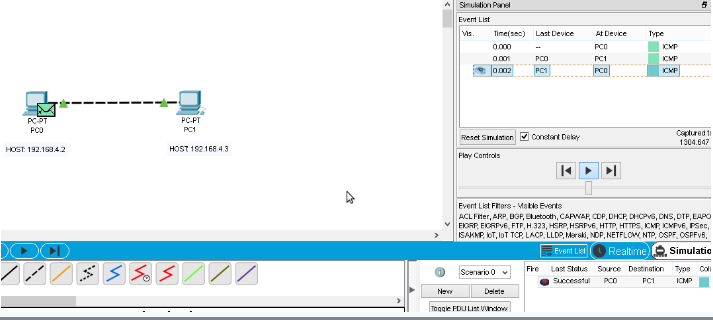
\includegraphics[scale=0.5]{a1}
\begin{definicion}[]{
 vemos que el env\'io es de manera directa entre cada computador
}
\end{definicion}

\subsection{Verifique la conectividad utilizando ping desde la l\'inea de comandos. Repita lo mismo entrando al modo de simulaci\'on.}
Entramos a desktop > command prompt > realizamos el ping
\\
\\
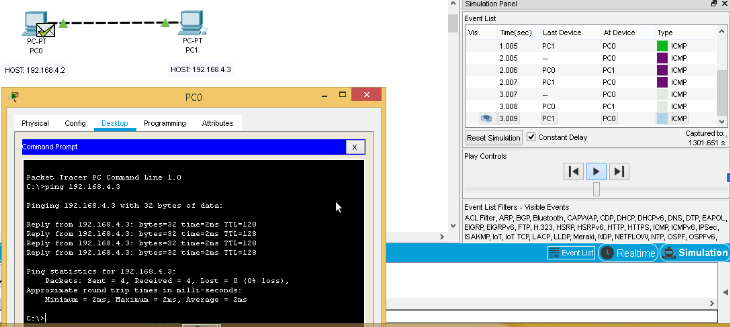
\includegraphics[scale=0.6]{ping}
\begin{definicion}[]
{
 vemos que entre las dos m\'aquinas hay comunicaci\'on de manera correcta.
}
\end{definicion}

\section{Red LAN: Un hub y 04 computadores}
\begin{caja}[]{
 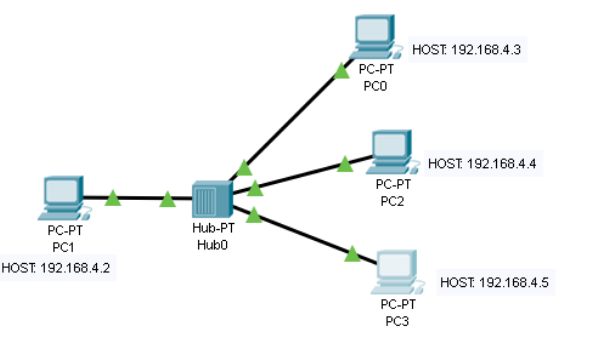
\includegraphics[scale=0.5]{2a} }
 \end{caja}
 
 
 \subsection{Simule el env\'io de un PDU entre la PC0 y PC2. Tome nota del comportamiento del hub.}
 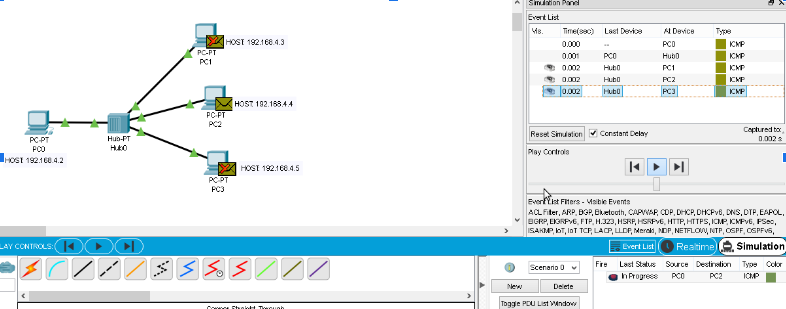
\includegraphics[scale=0.5]{hubpdu}
\begin{definicion}[]
{
 Se puede observar que el paquete viaja a todos los pcs y no solo a al computador destino; pero solo es tomado por el computador destino. Esto podr\'ia ser inseguro ya que todas las computadoras podr\'ian tener acceso al paquete.
}
\end{definicion}


 \subsection{Simule la ejecuci\'on del comando tracert (traceroute). Qu\'e diferencia observa en relaci\'on a la simulaci\'on de con ping}
 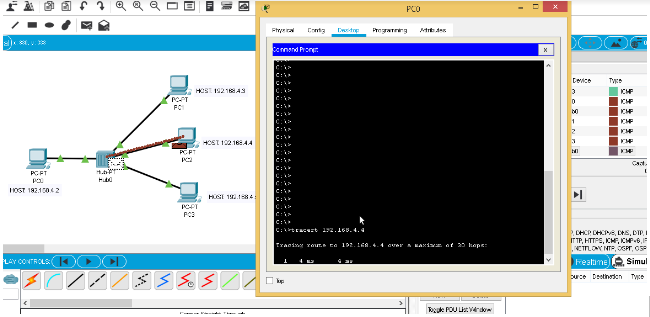
\includegraphics[scale=0.6]{tracert}
\begin{definicion}[]
{
 Al hacer el tracert se observa que demora m\'as y este comando te muestra el m\'inimo tiempo en que llega el paquete y el m\'aximo tiempo.
}
\end{definicion} 


\section{EJERCICIO 1}
\begin{definicion}[]{
Cree una red LAN con dos segmentos de red, donde cada segmento
de red tenga 01 hub y 04 computadoras y est\'en interconectadas
de hub a hub.
}
\end{definicion}

\begin{caja}{
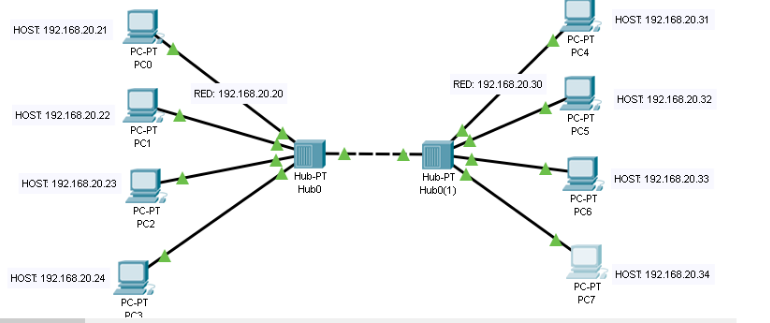
\includegraphics[scale=0.5]{ejercicio1}
}
\end{caja}

\subsection{Compruebe la ejecuci\'on de ping y tracert entre dos dispositivos del mismo segmento y dos dispositivos de segmentos diferentes.}
\subsubsection{Mismo segmento}
	\begin{enumerate}[label=\itembolasazules{}]
\item PING
\\
 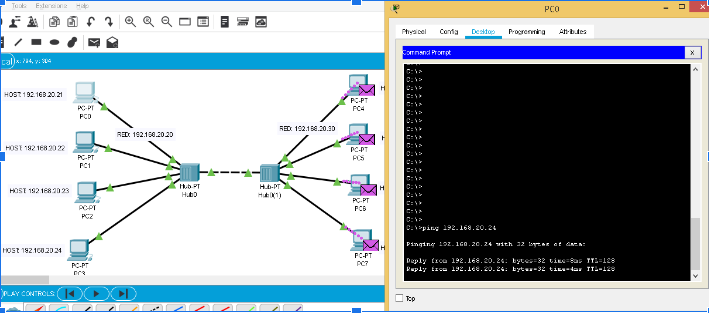
\includegraphics[scale=0.6]{ping1}
\begin{definicion}[]
{
Se puede observar que si hay comunicaci\'on entre la PC0 y la PC3, pero los paquetes tambi\'en llegan al otro segmento del hub.
}
\end{definicion} 
\item TRACERT
\\
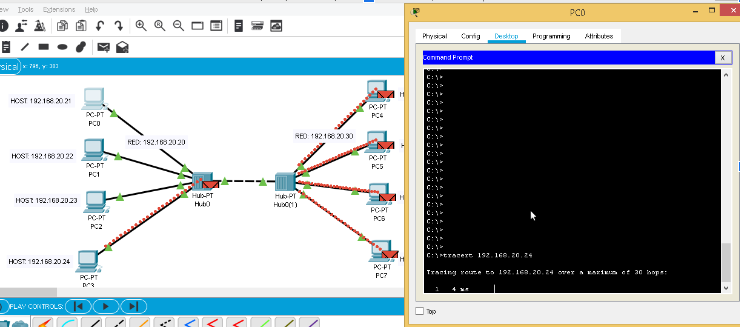
\includegraphics[scale=0.6]{tracert1}
\begin{definicion}[]
{
Se puede observar que la comunnicaci\'on demora mucho m\'as, ya que los paquetes tambi\'en viajan al otro segmento del hub.
}
\end{definicion} 
\end{enumerate}

\subsubsection{Segmentos diferentes}

\begin{enumerate}[label=\itembolasazules{}]
\item PING
\\
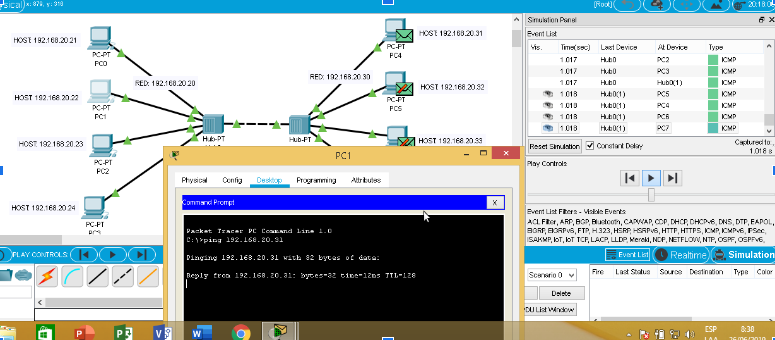
\includegraphics[scale=0.6]{ping2}
\begin{definicion}[]
{
se observa que si hay comunicaci\'on de un segmento a otro(PC1 A PC4).
}
\end{definicion} 
\end{enumerate}
\item TRACERT
\\
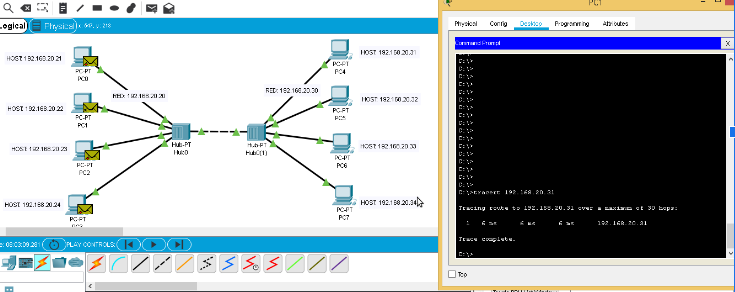
\includegraphics[scale=0.6]{tracert2}
\begin{definicion}[]
{
se observa que si que ahora se demora mucho m\'as).
}
\end{definicion} 
\end{enumerate}

\section{Simule el env\'io de paquetes entre dos hosts del mismo segmento y entre dos hosts de segmentos diferentes.}
\subsubsection{Mismo segmento}
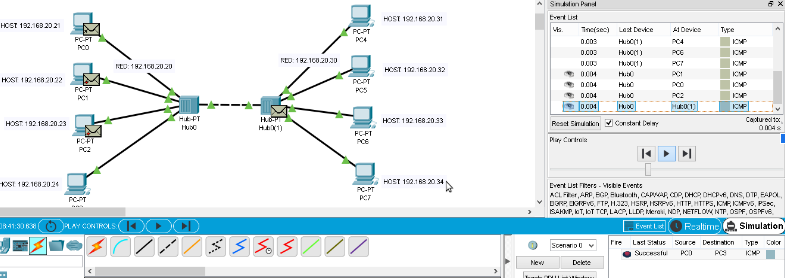
\includegraphics[scale=0.6]{pdu1}
\begin{definicion}[]
{
se observa que el paquete viaja a trav\'es de ambos hubs y llega a todas las m\'aquinas independientemente a quien estemos envi\'andolo
}
\end{definicion} 


\subsubsection{Segmentos diferentes}
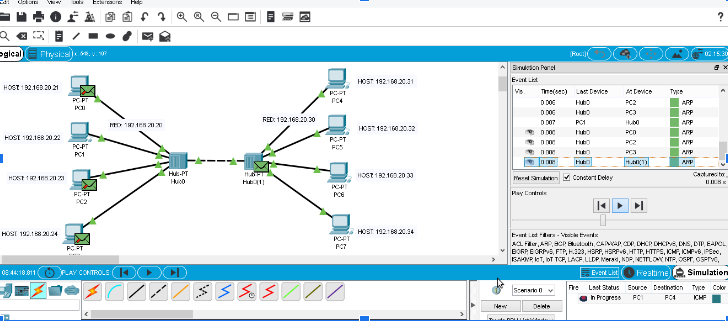
\includegraphics[scale=0.6]{pdu2}
\begin{definicion}[]
{
Al igual que el env\'io anterior el paquete viaja a trav\'es de ambos hubs y llega a todas las PC
}
\end{definicion} 

\subsection{Determine el dominio de colisi\'on}
\begin{definicion}[]
{
El dominio de colisi\'on en este caso ser\'ia toda la red ya que un hub lo que hace difundir el dominio de colisi\'on y no romper el dominio de colisi\'on como si lo hace un conmutador.
}
\end{definicion} 


\section{EJERCICIO 2}
%imagen
\begin{definicion}[]
{
Cree una red LAN con dos segmentos de red, donde un segmento
de red tenga 01 hub y 04 computadoras, mientras que el otro
tenga 04 computadores y est\'en interconectados a un switch. Los
segmentos de red, a su vez, est\'en interconectadas de hub a
switch.\\\\
Como direcciones IP, utilice el rango comprendido entre
192.160.10.50 y 192.160.10.60
}
\end{definicion} 
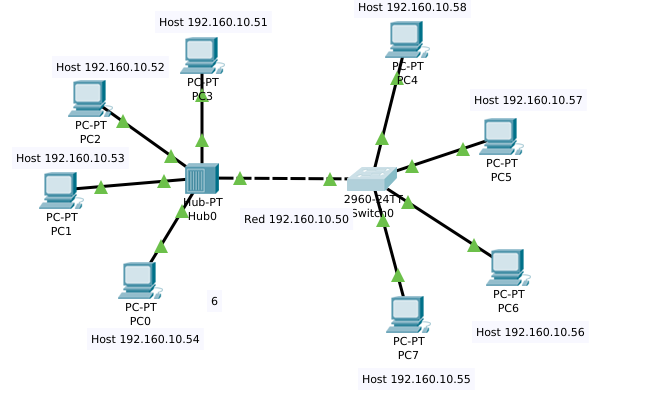
\includegraphics[scale=0.5]{img/dosswitchs.png}
\\\begin{center}
La construcci\'on de la red seria asi.
\end{center}
\subsubsection{Compruebe la ejecuci\'on de ping y tracert entre los distintos nodos de red, adem\'as de simular el env\'io de paquetes simples y complejos entre los distintos nodos.}
\textit{simulamos que todos los nodos se conectan correctamente:}\\

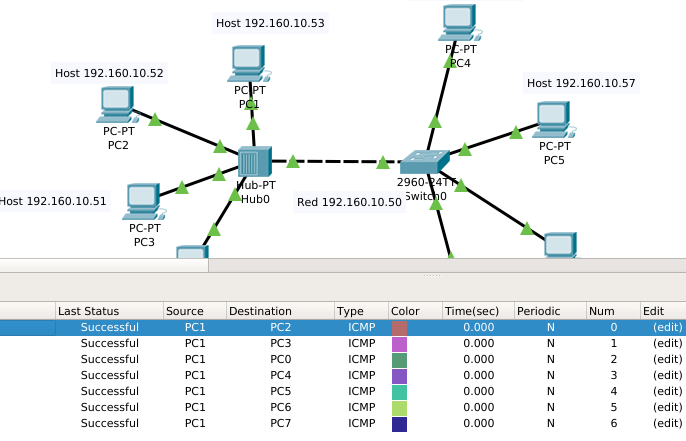
\includegraphics[scale=0.5]{img/prueba1.png} \\
%imagen
%descripcion
\subsubsection{Simule el env\'io de paquetes entre dos hosts del mismo segmento y entre dos hosts de segmentos diferentes.}
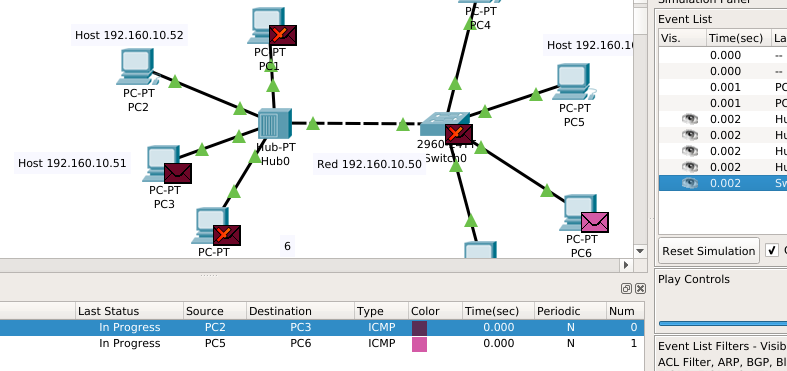
\includegraphics[scale=0.5]{img/simulacion1.png} \\
Como se puede observar el comportamiendo del hub es enviar los paquetes a todos, mientras que el switch no realiza esta acci\'on\\
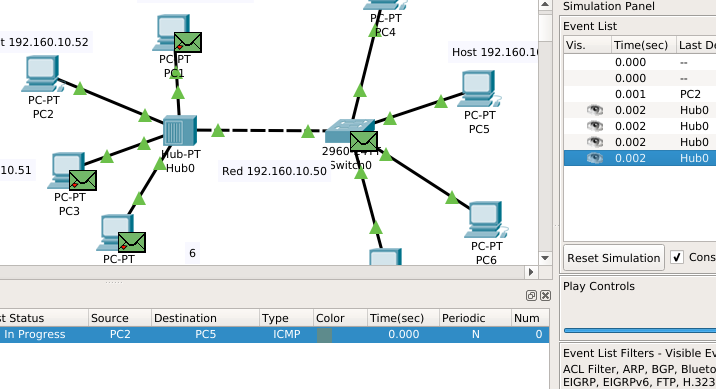
\includegraphics[scale=0.5]{img/simulacion2.png} \\
Para el caso de diferentes segmentos lo que hace el hub es lo mismo que lo anterior.
%imagen
%descripcion
\subsubsection{Determine el dominio de colisi\'on.}
En total hay 5 dominios de colisi\'on ya que un conmmutador rompe el dominio de colisi\'on.
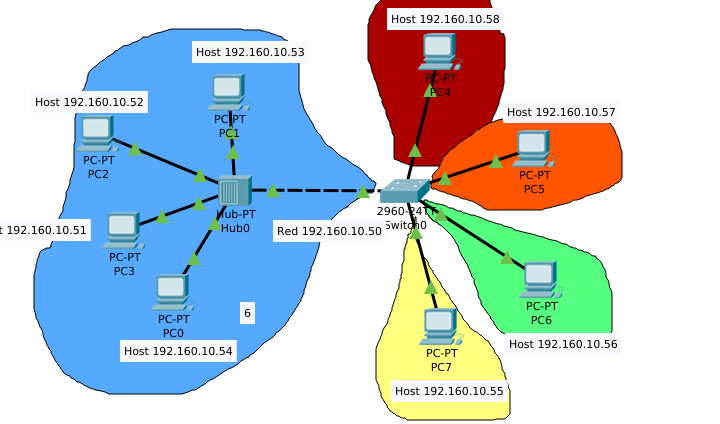
\includegraphics[scale=0.6]{img/dominio.png} 


\section{Red LAN: Switch y 03 Servidores}
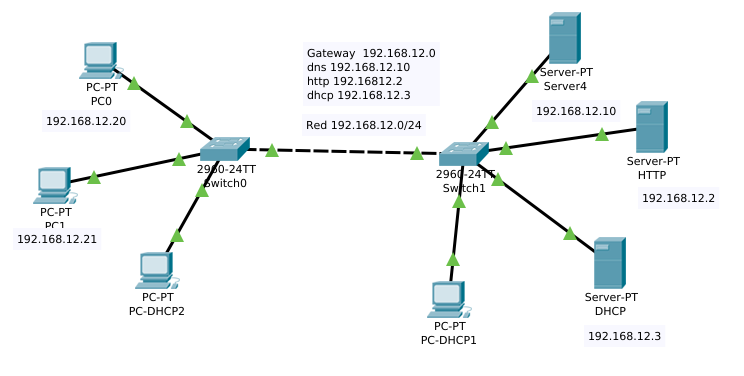
\includegraphics[scale=0.45]{img/switch3ser.png} 
\begin{definicion}[]
{
Hacer ping desde cada una de las PCs al servidor HTTP y
probar el acceso a una p\'agina web dise\~nada por su persona.
}
\end{definicion} 
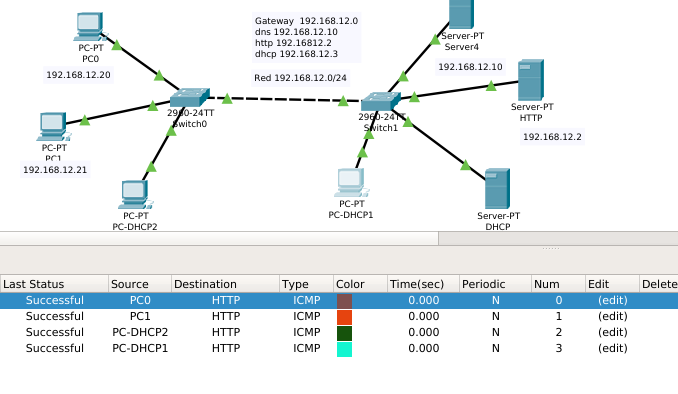
\includegraphics[scale=0.5]{img/pinghttp.png} \\
En este caso lo que hacemos es mandar paquetes para ver si hay conexi\'on por lo que observamos la conexi\'on a sido exitosa.
\\probando que el servidor http funcione\\
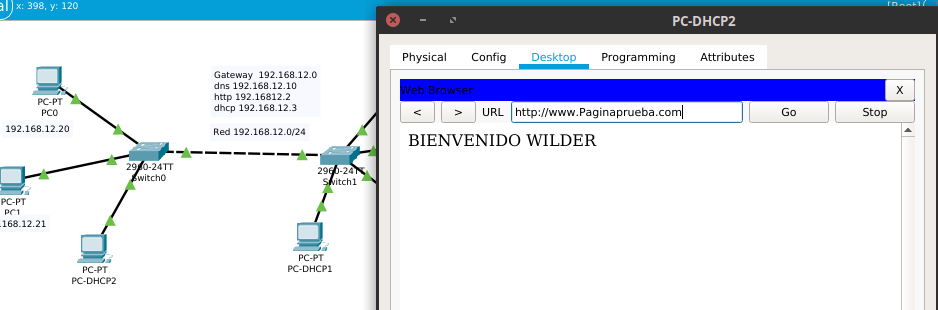
\includegraphics[scale=0.5]{img/prueba.png} \\
el servidor http esta respondiendo de manera adecuada.\\
las configuraciones que hicimos fueron:\\
\textbf{dns}\\
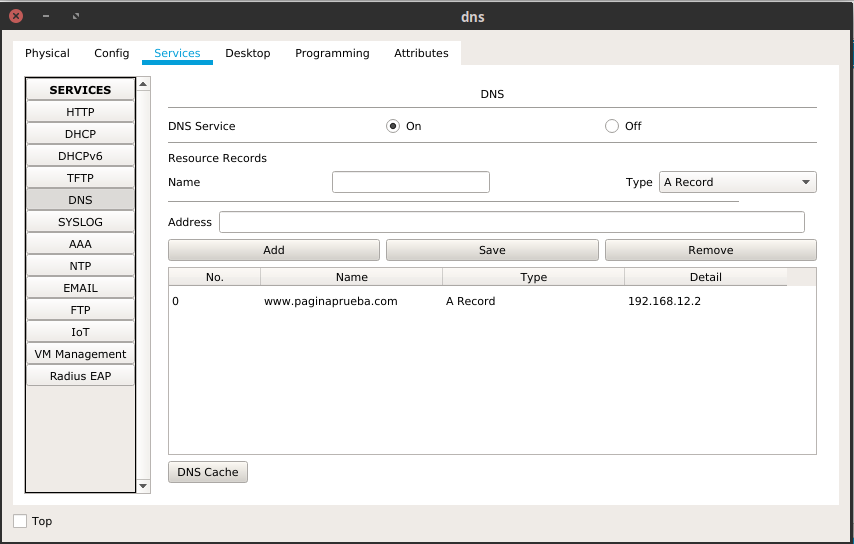
\includegraphics[scale=0.5]{img/dns.png} 
\\En el servidor dns establecemos como ah de llamarse nuestra web a mostrar.\\
\textbf{http}\\
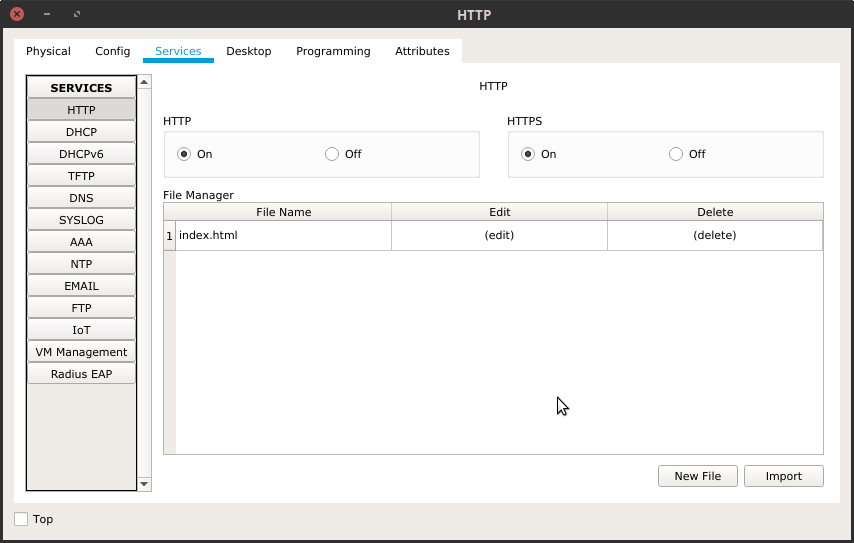
\includegraphics[scale=0.5]{img/http.png}
\\En este servidor configuramos la pagina a mostrar\\
\textbf{dhcp}\\
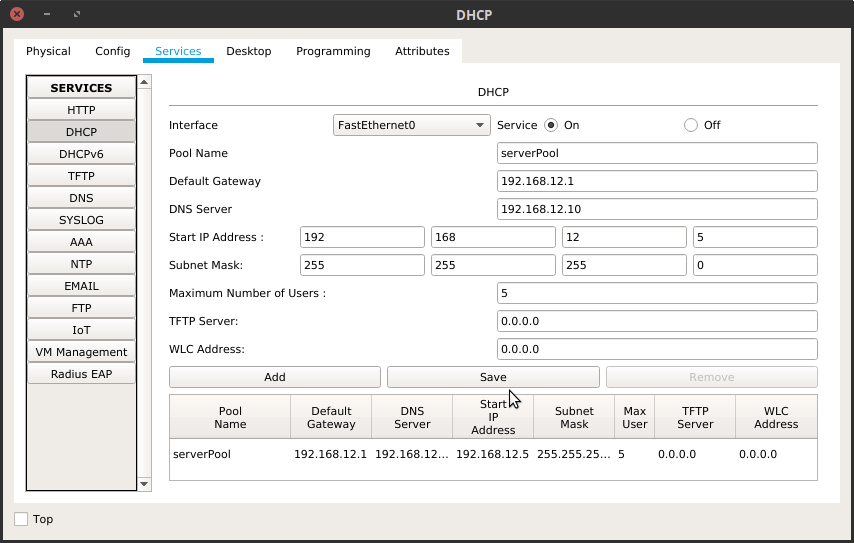
\includegraphics[scale=0.5]{img/dhcp.png} 
\\En este servidor configuramos la ip dinamica que van a recibir las pcs
\\
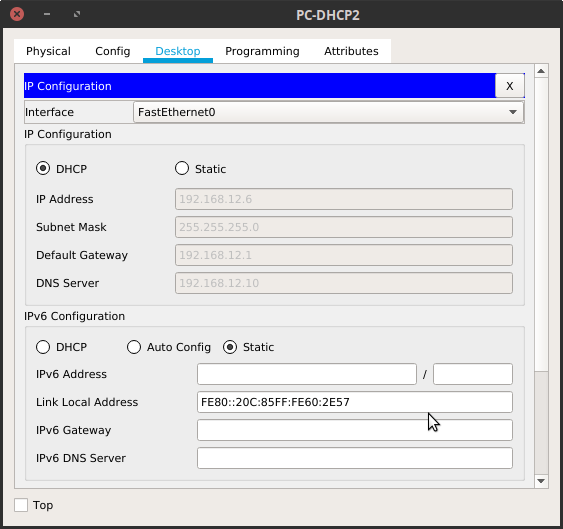
\includegraphics[scale=0.5]{img/dhcpejem.png} 

\section{caso}
Se presenta implementar una web universitaria de conferencias a la cual puedan visitar los alumnos de civil, minas y biologia.\\

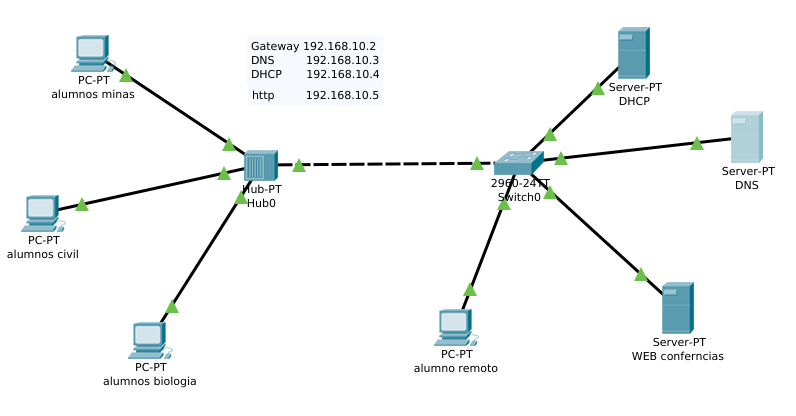
\includegraphics[scale=0.5]{img/confe.png} 
\\ vemos que los alumnos ingresan:\\
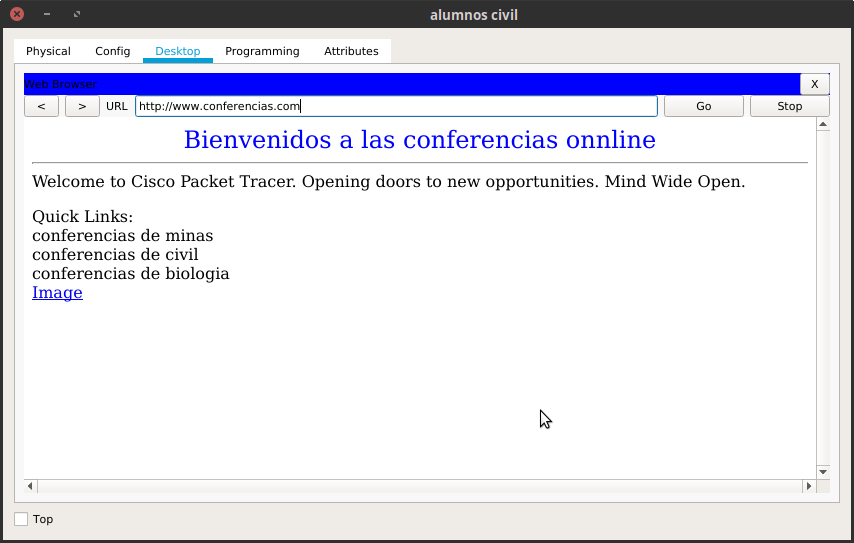
\includegraphics[scale=0.5]{img/civil.png} 
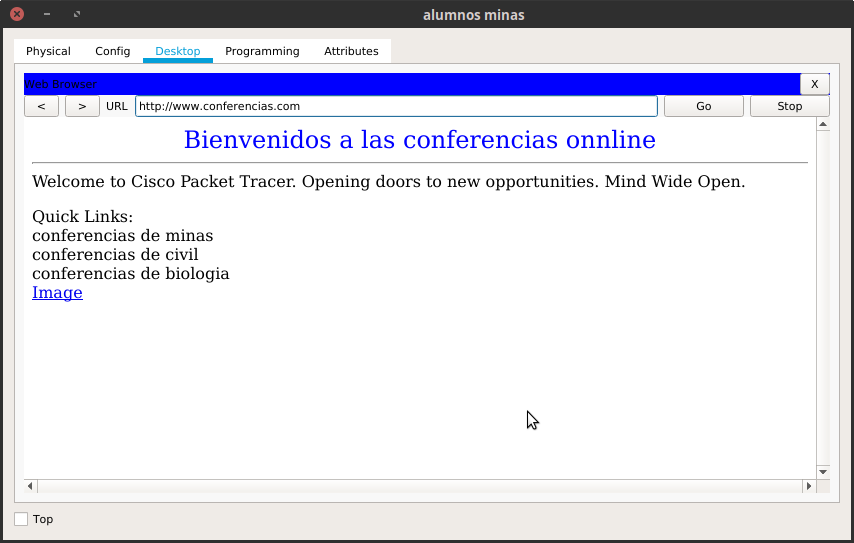
\includegraphics[scale=0.5]{img/minas.png} 
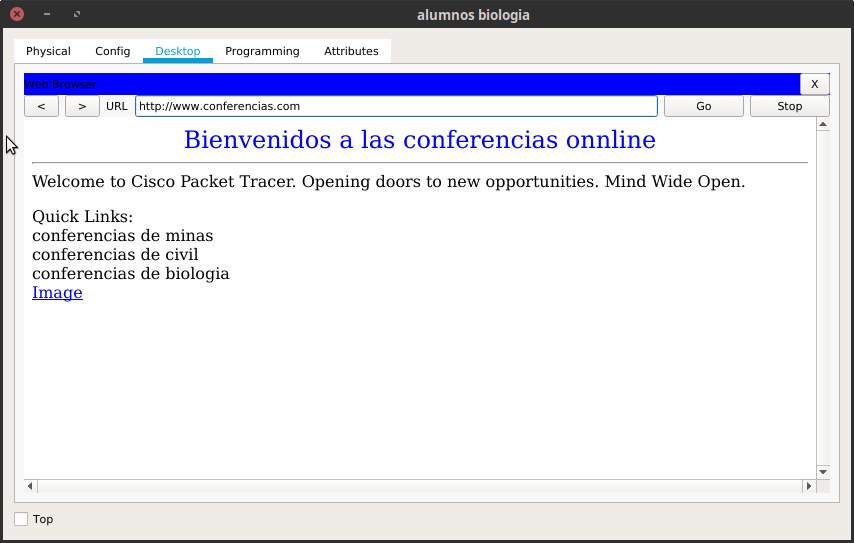
\includegraphics[scale=0.5]{img/biologia.png} 
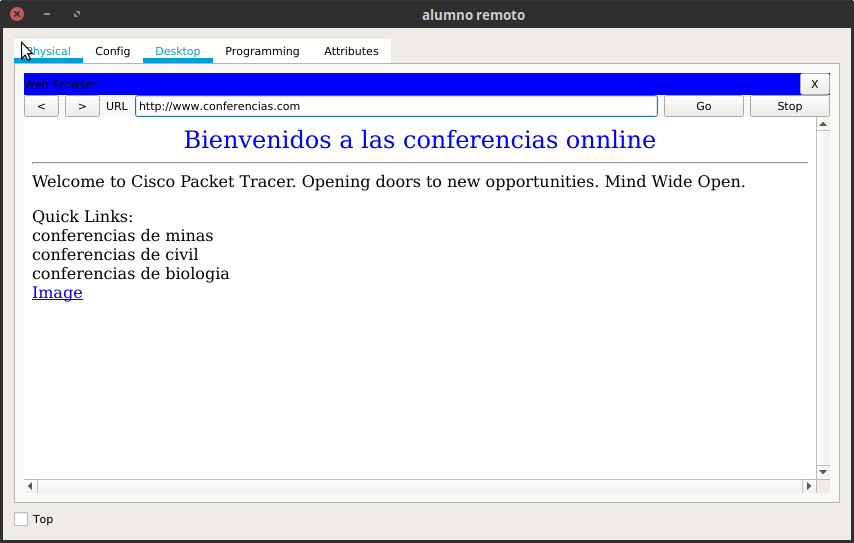
\includegraphics[scale=0.5]{img/otros.png} 